% Created 2014-08-26 Tue 18:53
\documentclass[bigger]{beamer}
\usepackage[utf8]{inputenc}
\usepackage[T1]{fontenc}
\usepackage{fixltx2e}
\usepackage{graphicx}
\usepackage{longtable}
\usepackage{float}
\usepackage{wrapfig}
\usepackage{soul}
\usepackage{textcomp}
\usepackage{marvosym}
\usepackage{wasysym}
\usepackage{latexsym}
\usepackage{amssymb}
\usepackage{hyperref}
\tolerance=1000
\mode<beamer>{\usetheme[compress]{Berlin}}
\usepackage{graphicx}
\usepackage{amsmath}
\usepackage{lmodern}
\usepackage{ifmtarg}
\usepackage{tikz}
\usetikzlibrary{calc}
\makeatletter
\newcommand\ChangeItemFont[3]{%
\renewcommand{\itemize}[1][]{%
  \beamer@ifempty{##1}{}{\def\beamer@defaultospec{#1}}%
  \ifnum \@itemdepth >2\relax\@toodeep\else
    \advance\@itemdepth\@ne
    \beamer@computepref\@itemdepth% sets \beameritemnestingprefix
    \usebeamerfont{itemize/enumerate \beameritemnestingprefix body}%
    \usebeamercolor[fg]{itemize/enumerate \beameritemnestingprefix body}%
    \usebeamertemplate{itemize/enumerate \beameritemnestingprefix body begin}%
    \list
      {\usebeamertemplate{itemize \beameritemnestingprefix item}}
      {\def\makelabel####1{%
          {%
            \hss\llap{{%
                \usebeamerfont*{itemize \beameritemnestingprefix item}%
                \usebeamercolor[fg]{itemize \beameritemnestingprefix item}####1}}%
          }%
        }%
  \ifnum\@itemdepth=1\relax
    #1%
  \else
  \ifnum\@itemdepth=2\relax
    #2%
  \else
  \ifnum\@itemdepth=3\relax
    #3%
  \fi%
  \fi%
  \fi%
  }
  \fi%
  \beamer@cramped%
  \raggedright%
  \beamer@firstlineitemizeunskip%
}}
\makeatother

\setbeamertemplate{footline}
  {%
    \begin{beamercolorbox}[colsep=1.5pt]{upper separation line foot}
    \end{beamercolorbox}
    \begin{beamercolorbox}[ht=2.5ex,dp=1.125ex,%
      leftskip=.3cm,rightskip=.3cm plus1fil]{author in head/foot}%
      \leavevmode{\usebeamerfont{author in head/foot}\insertshortauthor}%
      \hfill%
      {\usebeamerfont{institute in head/foot}\usebeamercolor[fg]{institute in head/foot}\insertshortinstitute}%
    \end{beamercolorbox}%
    \begin{beamercolorbox}[ht=2.5ex,dp=1.125ex,%
      leftskip=.3cm,rightskip=.3cm plus1fil]{title in head/foot}%
      {\usebeamerfont{title in head/foot}\insertshorttitle}%
      \hfill%
      {\usebeamerfont{frame number}\usebeamercolor[fg]{frame number}\insertframenumber~/~\inserttotalframenumber}
    \end{beamercolorbox}%
    \begin{beamercolorbox}[colsep=1.5pt]{lower separation line foot}
    \end{beamercolorbox}
  }
\makeatother


%----------------------------------------------------------------------
% Define useful commands
%----------------------------------------------------------------------

\newcommand{\eejj}{\ensuremath{eejj} }
\newcommand{\enujj}{\ensuremath{e\nu jj} }
\newcommand{\mumujj}{\ensuremath{\mu\mu jj} }
\newcommand{\munujj}{\ensuremath{\mu\nu jj} }
\newcommand{\emujj}{\ensuremath{e\mu jj} }
\newcommand{\zjets}{\ensuremath{\text{Z}^{0}}+jets }
\newcommand{\wjets}{\ensuremath{\text{W}^{\pm}}+jets }
\newcommand{\ttbar}{\ensuremath{t\bar{t}} }

\newcommand{\pt}{\ensuremath{p_{\text{T}}} }
\newcommand{\ST}{\ensuremath{S_{\text{T}}} }
\newcommand{\mee}{\ensuremath{m_{\text{ee}}} }
\newcommand{\mll}{\ensuremath{m_{\ell\ell}} }
\newcommand{\mej}{\ensuremath{m_{\text{ej}}} }
\newcommand{\mejmin}{\ensuremath{m_{\text{ej}}^{\text{min}}} }
\newcommand{\mejavg}{\ensuremath{m_{\text{ej}}^{\text{avg}}} }
% \newcommand{\mt}{\ensuremath{m_{\text{T, e}\nu}}}
\newcommand{\mtjnu}{\ensuremath{m_{\text{T, j}\nu}} }


\newcommand{\met}{\ensuremath{\not\!\!{E_{\text{T}}}} }
\newcommand{\mt}{\ensuremath{m_{\text{T, e}\nu}} }

%----------------------------------------------------------------------
% Define useful numbers
%----------------------------------------------------------------------

% Lumi info
\newcommand{\intLumi}{$19.6 \text{ fb}^{-1}$}

% MC scale factors
\newcommand{\enujjWJetsMonteCarloScaleFactor}{0.85 \pm 0.01 \text{ (stat)} \pm 0.01    \text{ (syst)}}
\newcommand{\enujjTTBarMonteCarloScaleFactor}{0.97 \pm 0.02 \text{ (stat)} \pm 0.01    \text{ (syst)}}
% \newcommand{\eejjZJetsMonteCarloScaleFactor} {0.97 \pm 0.01 \text{ (stat)} \pm 0.00004 \text{ (syst)}}
\newcommand{\eejjZJetsMonteCarloScaleFactor} {0.97 \pm 0.01 \text{ (stat)}}

\newcommand{\enujjWJetsMonteCarloScaleFactorMETRescaled}{0.95 \pm 0.02 \text{ (stat)} \pm 0.01 \text{ (syst)}}
\newcommand{\enujjTTBarMonteCarloScaleFactorMETRescaled}{1.07 \pm 0.03 \text{ (stat)} \pm 0.01 \text{ (syst)}}

\newcommand{\enujjWJetsMonteCarloScaleFactorMETandMTRescaled}{0.97 \pm 0.02 \text{ (stat)} \pm 0.01 \text{ (syst)}}
\newcommand{\enujjTTBarMonteCarloScaleFactorMETandMTRescaled}{1.08 \pm 0.03 \text{ (stat)} \pm 0.01 \text{ (syst)}}

\newcommand{\eejjZControlRegionContamination}{4\%}

% Electron scale factors
\newcommand{\electronRecoDataMCScaleFactor}{0.98}
\newcommand{\electronRecoDataMCScaleFactorRelUnc}{1.5}
\newcommand{\electronRecoDataMCScaleFactorSqr}{0.96}

% GEN-level cross-sections (not yet rescaled) 
\newcommand{\wjetsXSection}{37509.0 pb}
\newcommand{\zjetsXSection}{3503.71 pb}
\newcommand{\ttbarXSection}{234 pb}
\newcommand{\stopSChannelXSection}{5.55 pb}
\newcommand{\stopTChannelXSection}{87.1 pb}
\newcommand{\stopTWChannelXSection}{22.2 pb}
\newcommand{\wwXSection}{57.1 pb} % THESE NEED TO BE UPDATED!!!
\newcommand{\wzXSection}{32.3 pb} % THESE NEED TO BE UPDATED!!!
\newcommand{\zzXSection}{8.26 pb} % THESE NEED TO BE UPDATED!!!

% QCD contributions at limit of the analysis
\newcommand{\percentQCDatEEJJLimit}{1\%}
\newcommand{\percentQCDatENuJJLimit}{3\%}

% Closure test contamination
\newcommand{\percentContaminationClosureTest}{5\%}
\newcommand{\percentContaminationClosureTestFinal}{55\%}

% Closure test (low-ST) results
\newcommand{\closureTestLowSTPredicted}{13100}
\newcommand{\closureTestLowSTPredictedUnc}{400}
\newcommand{\closureTestLowSTObserved}{12100}
\newcommand{\closureTestLowSTObservedUnc}{400}
\newcommand{\closureTestLowSTRatio}{1.08}
\newcommand{\closureTestLowSTRatioUnc}{0.05}

% Closure test (mid-ST) results
\newcommand{\closureTestMidSTPredicted}{877}
\newcommand{\closureTestMidSTPredictedUnc}{46.7}
\newcommand{\closureTestMidSTObserved}{600}
\newcommand{\closureTestMidSTObservedUnc}{53}
\newcommand{\closureTestMidSTRatio}{1.46}
\newcommand{\closureTestMidSTRatioUnc}{0.15}

% QCD systematic uncertainty
\newcommand{\qcdSystematicUncertaintyPerEle}{30\%}
\newcommand{\qcdSystematicUncertaintyTwoEle}{60\%}

% TTbar (e-mu-jj) contamination
\newcommand{\emujjContamination}{2\%}
\newcommand{\emujjRecoScaleFactor}{0.974  \pm 0.011 \text{ (stat)}}

% mumujj/munujj scale factors for data-driven background
\newcommand{\mumujjRecoScaleFactor}{97.5 \pm 0.4 \text{ (stat)}}
\newcommand{\munujjRecoScaleFactor}{97.2 \pm 0.5 \text{ (stat)}}

% Shape uncertainties
\newcommand{\enujjWJetsShapeUncertainty}{5.92\%}
\newcommand{\enujjTTBarShapeUncertainty}{8.17\%}
\newcommand{\eejjZJetsShapeUncertainty}{8.70\%}

% EES uncertainties
\newcommand{\electronEnergyScaleUncBarrel}{0.4\%}
\newcommand{\electronEnergyScaleUncEndcap}{4.1\%}

% EER uncertainties
\newcommand{\electronEnergyResolutionUncBarrel}{1.006}
\newcommand{\electronEnergyResolutionUncEndcap}{1.015}

% lumi uncertainty
\newcommand{\lumiUncertainty}{2.6\%}

% limits
\newcommand{\eejjObservedLimit}{1005}
\newcommand{\eejjExpectedLimit}{1030}
\newcommand{\enujjObservedLimit}{845}
\newcommand{\enujjExpectedLimit}{890}

\newcommand{\enujjObservedLimitCombined}{845}
\newcommand{\enujjExpectedLimitCombined}{932}

\newcommand{\eejjObservedLimitNoSyst}{1010}
\newcommand{\eejjExpectedLimitNoSyst}{1030}
\newcommand{\enujjObservedLimitNoSyst}{850}
\newcommand{\enujjExpectedLimitNoSyst}{895}

\newcommand{\eejjObservedLimitMuon}{1015}
\newcommand{\eejjExpectedLimitMuon}{980}
\newcommand{\enujjObservedLimitMuon}{825}
\newcommand{\enujjExpectedLimitMuon}{890}


\newcommand{\lowBetaExpectedLimit}{790}
\newcommand{\lowBetaObservedLimit}{635}

\mode<beamer>{\usecolortheme{bear}}
\mode<beamer>{\titlegraphic{\includegraphics[width=0.2\textwidth]{brown-logo}}}
\institute[Brown University]{}
\AtBeginSection{\frame{\sectionpage}}
\providecommand{\alert}[1]{\textbf{#1}}

\title{HCAL developments for Jets and MET}
\author{Edmund Berry}
\date{Friday, August 22, 2014}
\hypersetup{
  pdfkeywords={},
  pdfsubject={},
  pdfcreator={Emacs Org-mode version 7.8.11}}

\author[Edmund A. Berry]{\alert{Edmund A. Berry}}
\begin{document}

\maketitle


\section{Introduction}
\label{sec-1}
\subsection{Introduction}
\label{sec-1-1}
\begin{frame}
\frametitle{Introduction}
\label{sec-1-1-1}
\begin{itemize}

\item Changes between the Run 1 and Run 2 physics environments are well-documented
\label{sec-1-1-1-1}%

\item HCAL has implemented hardware upgrades in response
\label{sec-1-1-1-2}%

\item Software updates must:
\label{sec-1-1-1-3}%
\begin{itemize}

\item Account for hardware changes (e.g. recalibration)
\label{sec-1-1-1-3-1}%

\item Respond to physics changes in Run 2 environment
\label{sec-1-1-1-3-2}%
\end{itemize} % ends low level
\end{itemize} % ends low level
\end{frame}
\begin{frame}
\frametitle{HCAL hardware upgrades during LS1}
\label{sec-1-1-2}
\begin{itemize}

\item HB and HE:
\label{sec-1-1-2-1}%
\begin{itemize}

\item Replaced clock, control, monitor modules
\label{sec-1-1-2-1-1}%

\item \alert{Removes synchronization problems with isolated sections of HB and HE}
\label{sec-1-1-2-1-2}%
\end{itemize} % ends low level

\item HO
\label{sec-1-1-2-2}%
\begin{itemize}

\item Changed hybrid photodiodes to silicon photomultipliers
\label{sec-1-1-2-2-1}%

\item \alert{Improves signal to noise for MIPs in HO}
\label{sec-1-1-2-2-2}%
\end{itemize} % ends low level

\item HF
\label{sec-1-1-2-3}%
\begin{itemize}

\item Replaced single-anode photomultiplier tubes (PMTs) with thin window multi-anode PMTs
\label{sec-1-1-2-3-1}%

\item Also: installed new cables capable of dual readout
\label{sec-1-1-2-3-2}%

\item \alert{Reduces fake signal from PMT window hits}
\label{sec-1-1-2-3-3}%
\end{itemize} % ends low level
\end{itemize} % ends low level
\end{frame}
\begin{frame}
\frametitle{HCAL software responses}
\label{sec-1-1-3}

\centering
HCAL software is responding in many ways, \\
all of which affect jets and MET
\begin{block}{I will discuss three in particular:}
\label{sec-1-1-3-1}

\begin{enumerate}
\item Calibration
\item Reconstruction
\item Noise filters
\end{enumerate}
\end{block}
\end{frame}
\section{Calibration}
\label{sec-2}
\subsection{Introduction to calibration}
\label{sec-2-1}
\begin{frame}
\frametitle{Calibration scope and priorities}
\label{sec-2-1-1}
\begin{itemize}

\item Tuning and development (\alert{now - end 2014})
\label{sec-2-1-1-1}%
\begin{itemize}

\item Address HCAL shortcomings revealed during Run 1
\label{sec-2-1-1-1-1}%

\item Tune existing Run 1 methods for Run 2 environment
\label{sec-2-1-1-1-2}%

\item Develop new methods when necessary
\label{sec-2-1-1-1-3}%
\end{itemize} % ends low level

\item Preparing HCAL pre-calibration, (\alert{end 2014, 2 months})\\
\label{sec-2-1-1-2}%
Relying on:
\begin{itemize}

\item Radioactive source calibration: critical for HF startup calibration
\label{sec-2-1-1-2-1}%

\item Cosmics: very effective tool for HO calibration
\label{sec-2-1-1-2-2}%

\item Splashes: useful in 2009 and 2010 for HBHE, not essential in 2015
\label{sec-2-1-1-2-3}%
\end{itemize} % ends low level

\item Integration of HCAL tools with AlCa (\alert{\texttt{CMSSW\_7\_3\_X}})
\label{sec-2-1-1-3}%
\begin{itemize}

\item \alert{If necessary}
\label{sec-2-1-1-3-1}%
\end{itemize} % ends low level
\end{itemize} % ends low level
\end{frame}
\begin{frame}
\frametitle{Calibration outline}
\label{sec-2-1-2}
\begin{block}{Three main areas of focus:}
\label{sec-2-1-2-1}

\begin{enumerate}
\item Radiation damage correction
\item $\phi$ symmetry calibration
\item Absolute energy calibration:
\begin{itemize}
\item HB \& part of HE: single particle (IsoTracks)
\item HE (\& perhaps elsewhere): dijet, $\gamma$-jet
\item HF: $Z\rightarrow ee$
\item HO: muons (GeV/MIP sets the scale)
\end{itemize}
\end{enumerate}
\end{block}
\begin{itemize}

\item Conveners: \href{mailto:jordan.damgov@cern.ch}{\underline{\alert{Jordan Damgov}}} and \href{mailto:yurii.maravin@cern.ch}{\underline{\alert{Yurii Maravin}}}
\label{sec-2-1-2-2}%
\end{itemize} % ends low level
\end{frame}
\subsection{Radiation damage correction}
\label{sec-2-2}
\begin{frame}
\frametitle{Radiation damage in the HE: what we know today}
\label{sec-2-2-1}
\begin{columns} % Columns
\label{sec-2-2-1-1}
\begin{column}{0.55\textwidth}
%% Text column
\label{sec-2-2-1-1-1}
\begin{itemize}

\item In first 20 $\text{fb}^{-1}$, in the high-$\eta$ region ($|\eta| = 3$)
\label{sec-2-2-1-1-1-1}%
\begin{itemize}

\item L1 lost 30\% orig. signal
\label{sec-2-2-1-1-1-1-1}%

\item L7 lost 15\% orig. signal
\label{sec-2-2-1-1-1-1-2}%
\end{itemize} % ends low level

\item Even at $|\eta = 2.4|$ the loss was non-negligible
\label{sec-2-2-1-1-1-2}%
\begin{itemize}

\item L1 lost 15\% orig. signal
\label{sec-2-2-1-1-1-2-1}%

\item L7 lost  5\% orig. signal
\label{sec-2-2-1-1-1-2-2}%
\end{itemize} % ends low level
\end{itemize} % ends low level
\end{column}
\begin{column}{0.55\textwidth}
%% HE
\label{sec-2-2-1-1-2}

\centering
Results for Layer 1 of HE
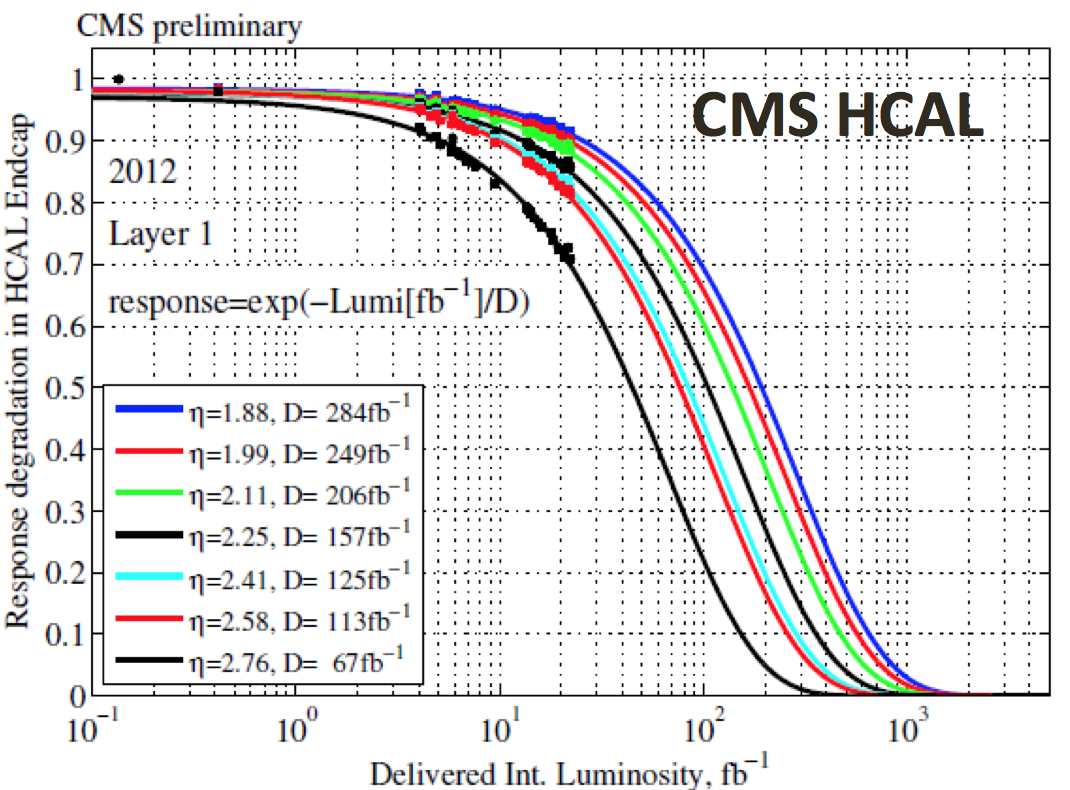
\includegraphics[width=\textwidth]{fig/radHE.png}
\end{column}
\end{columns}
\begin{itemize}

\item Raddam work: \href{mailto:Robert.Ciesielski@cern.ch}{\underline{\alert{R. Ciesielski}}}, \href{mailto:vladimir.epshteyn@cern.ch}{\underline{\alert{V. Epshteyn}}}, \href{mailto:dmitry.vishnevskiy@cern.ch}{\underline{\alert{D. Vishnevskiy}}}
\label{sec-2-2-1-2}%
\end{itemize} % ends low level
\end{frame}
\begin{frame}
\frametitle{Radiation damage in the HE: how we know it}
\label{sec-2-2-2}
\begin{columns} % Columns
\label{sec-2-2-2-1}
\begin{column}{0.55\textwidth}
%% Text column
\label{sec-2-2-2-1-1}
\begin{itemize}

\item In Run 1, radiation damage was monitored with laser measurements
\label{sec-2-2-2-1-1-1}%

\item In 2012, an additional method using pp data with physics triggers was introduced
\label{sec-2-2-2-1-1-2}%
\end{itemize} % ends low level
\end{column}
\begin{column}{0.55\textwidth}
%% Figure column
\label{sec-2-2-2-1-2}

\centering
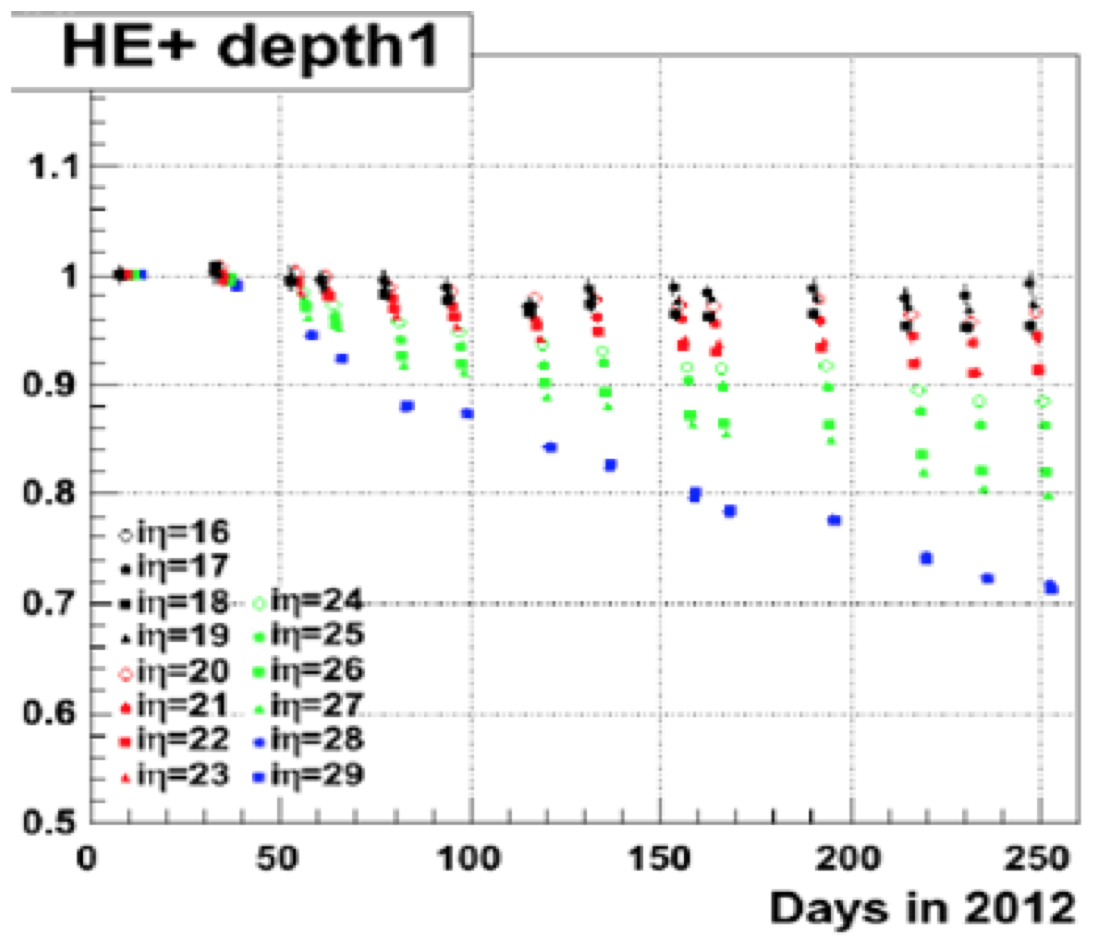
\includegraphics[width=.9\linewidth]{fig/HElaser.png}
\end{column}
\end{columns}
\end{frame}
\begin{frame}
\frametitle{Radiation damage in the HB: what we know today}
\label{sec-2-2-3}
%% Figure
\label{sec-2-2-3-1}

\centering
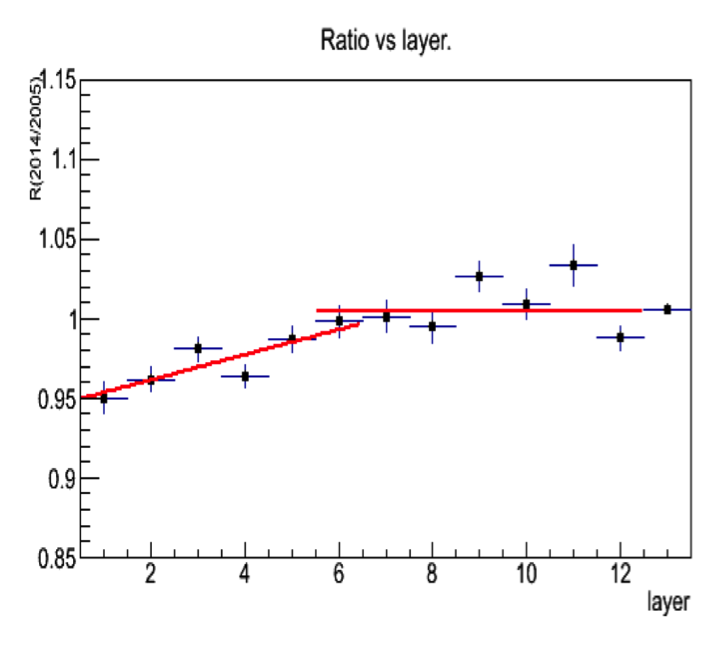
\includegraphics[width=0.50\textwidth]{fig/radHB.png}
\begin{itemize}

\item Ratio of signal from HB Co-60 calibration (2014/2005)
\label{sec-2-2-3-2}%

\item $2 \times 20^{\circ}$ wedges on HB-: \alert{April, 2014}
\label{sec-2-2-3-3}%

\item Consistent with 5\% damage to L1 of HB
\label{sec-2-2-3-4}%
\end{itemize} % ends low level
\end{frame}
\begin{frame}
\frametitle{Radiation damage in the HB: how we know it}
\label{sec-2-2-4}
%% Figure
\label{sec-2-2-4-1}

\centering
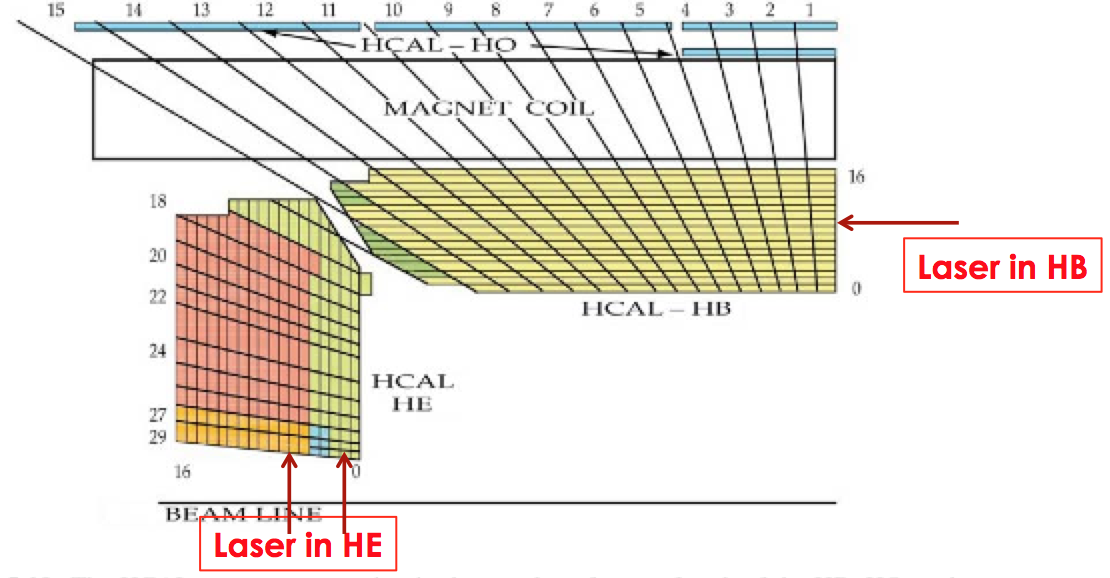
\includegraphics[width=0.7\textwidth]{fig/laserInsert.png}
\begin{itemize}

\item Laser monitoring can't monitor radiation damage to front layers of HB
\label{sec-2-2-4-2}%

\item Co-60 calibration (2005, 2014) is the only way to learn about radiation damage to front layers of HB
\label{sec-2-2-4-3}%
\end{itemize} % ends low level
\end{frame}
\begin{frame}
\frametitle{Radiation damage in the HB: how to deal with it}
\label{sec-2-2-5}
%% Figure
\label{sec-2-2-5-1}

\centering
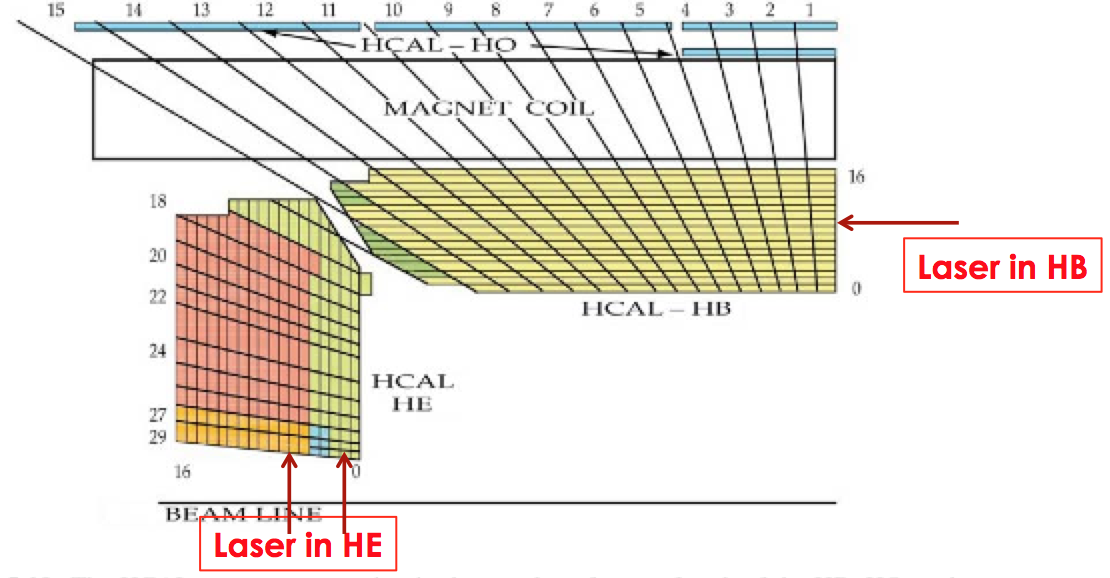
\includegraphics[width=0.7\textwidth]{fig/laserInsert.png}
\begin{itemize}

\item More data needed to establish effect beyond stat. fluct.
\label{sec-2-2-5-2}%

\item Since HB only has 1 depth (unlike HE with 2-3 depths), layer-dependent damage can only be corrected on average, introducing an energy dependence
\label{sec-2-2-5-3}%

\item Effect can probably be removed by MC corrections.
\label{sec-2-2-5-4}%
\end{itemize} % ends low level
\end{frame}
\begin{frame}
\frametitle{Radiation damage: what to do about it}
\label{sec-2-2-6}
\begin{itemize}

\item Current plan for HE:
\label{sec-2-2-6-1}%
\begin{itemize}

\item Use updated laser measurement algo. and updated laser
\label{sec-2-2-6-1-1}%

\item Use pp data as a less-frequent cross-check
\label{sec-2-2-6-1-2}%

\item First year of Run 2: expect signal loss similar to Run 1
\label{sec-2-2-6-1-3}%
\end{itemize} % ends low level

\item Current plan for HB:
\label{sec-2-2-6-2}%
\begin{itemize}

\item Data suggests layer-dependent radiation damage at 5\%
\label{sec-2-2-6-2-1}%

\item More data needed to establish effect beyond stat. fluct.
\label{sec-2-2-6-2-2}%

\item Continue Co-60 sourcing campaign on HB (\alert{Friday})
\label{sec-2-2-6-2-3}%

\item 4 additional HB wedges to be sourced
\label{sec-2-2-6-2-4}%
\end{itemize} % ends low level

\item Correct 2015 data at all levels (L1, HLT, Offline)
\label{sec-2-2-6-3}%
\end{itemize} % ends low level
\end{frame}
\subsection{$\phi$ symmetry calibration}
\label{sec-2-3}
\begin{frame}
\frametitle{$\phi$ symmetry calibration}
\label{sec-2-3-1}
\begin{itemize}

\item Goal: equalize response in $\phi$ for $\eta$-rings with 2 methods:
\label{sec-2-3-1-1}%

\item Method of moments
\label{sec-2-3-1-2}%
\begin{itemize}

\item Non-zero-suppressed and non-HCAL triggers
\label{sec-2-3-1-2-1}%

\item Worse precision in the HB than iterative method
\label{sec-2-3-1-2-2}%

\item $\sim5$ million events yields $\sim2\%$ precision
\label{sec-2-3-1-2-3}%
\end{itemize} % ends low level

\item Iterative method
\label{sec-2-3-1-3}%
\begin{itemize}

\item non-HCAL physics triggers
\label{sec-2-3-1-3-1}%

\item Better precision in the HB than moments method
\label{sec-2-3-1-3-2}%

\item 60 million events yields: 1\% HB; 0.2-2.5\% HE; 0.3\% HF
\label{sec-2-3-1-3-3}%
\end{itemize} % ends low level

\item Work on both methods is ongoing for Run 2 environment
\label{sec-2-3-1-4}%
\end{itemize} % ends low level
\end{frame}
\subsection{Absolute energy calibration}
\label{sec-2-4}
\begin{frame}
\frametitle{Absolute HB/HE energy calibration: single particle}
\label{sec-2-4-1}
\begin{itemize}

\item Method for calibration with isolated tracks
\label{sec-2-4-1-1}%

\item Tracker provides precision momentum measurement
\label{sec-2-4-1-2}%

\item Require:
\label{sec-2-4-1-3}%
\begin{itemize}

\item Good quality tracks reaching ECAL and HCAL
\label{sec-2-4-1-3-1}%

\item Tracks are isolated w.r.t. ECAL energy and other tracks
\label{sec-2-4-1-3-2}%
\end{itemize} % ends low level

\item Preparing estimates on precision for Run 2 environment
\label{sec-2-4-1-4}%

\item No IsoTrack trigger coverage in high $\eta$ HE region
\label{sec-2-4-1-5}%
\end{itemize} % ends low level
\end{frame}
\begin{frame}
\frametitle{Absolute HE energy scale: dijet balancing}
\label{sec-2-4-2}
\begin{itemize}

\item Method for ring-by-ring calibration with dijet events
\label{sec-2-4-2-1}%

\item Building on work done by JP Chou (\href{https://indico.cern.ch/event/75820/session/0/contribution/9/material/slides/0.pdf}{\underline{\alert{talk}}}, \href{http://cms.cern.ch/iCMS/jsp/openfile.jsp?type=IN&year=2008&files=IN2008_046.pdf}{\underline{\alert{IN2008/046}}})
\label{sec-2-4-2-2}%

\item Require:
\label{sec-2-4-2-3}%
\begin{itemize}

\item Two PFJets with small $|\Delta \eta|$: i.e. two PFJets in the same part of the jet energy response curve
\label{sec-2-4-2-3-1}%

\item Remove PU using PFJets
\label{sec-2-4-2-3-2}%
\begin{itemize}

\item Need to disambiguate energy corrections
\label{sec-2-4-2-3-2-1}%

\item Working with PF experts
\label{sec-2-4-2-3-2-2}%
\end{itemize} % ends low level
\end{itemize} % ends low level
\end{itemize} % ends low level
\end{frame}
\begin{frame}
\frametitle{Absolute HF energy scale: $Z\rightarrow ee$}
\label{sec-2-4-3}
\begin{columns} % Columns
\label{sec-2-4-3-1}
\begin{column}{0.55\textwidth}
%% Text
\label{sec-2-4-3-1-1}
\begin{itemize}

\item 2011 method: \href{http://cms.cern.ch/iCMS/jsp/openfile.jsp?type=DN&year=2011&files=DN2011_012.pdf}{\underline{\alert{DN2011/012}}}
\label{sec-2-4-3-1-1-1}%

\item Require:
\label{sec-2-4-3-1-1-2}%
\begin{itemize}

\item Precision tag electron in the ECAL with tracking
\label{sec-2-4-3-1-1-2-1}%

\item Probe electron in the HF
\label{sec-2-4-3-1-1-2-2}%
\end{itemize} % ends low level

\item For 2015 running:
\label{sec-2-4-3-1-1-3}%
\begin{itemize}

\item Special trigger needed to collect data at $|\eta| > 4.0$
\label{sec-2-4-3-1-1-3-1}%

\item Performance evaluated with CSA14 samples
\label{sec-2-4-3-1-1-3-2}%
\end{itemize} % ends low level
\end{itemize} % ends low level
\end{column}
\begin{column}{0.55\textwidth}
%% Plot
\label{sec-2-4-3-1-2}

\centering
Results from 2012
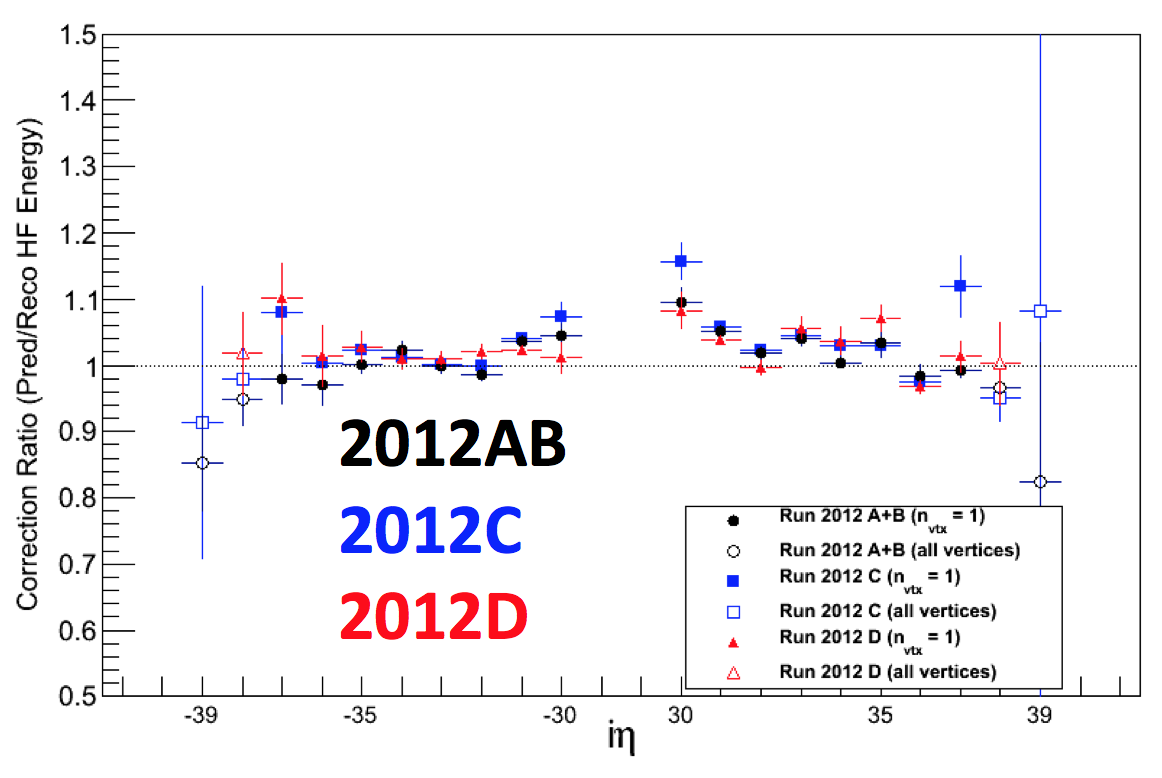
\includegraphics[width=\textwidth]{fig/HF_Zee.png}
\end{column}
\end{columns}
\end{frame}
\section{Reconstruction}
\label{sec-3}
\subsection{Introduction to reconstruction}
\label{sec-3-1}
\begin{frame}
\frametitle{Reconstruction scope and priorities}
\label{sec-3-1-1}
\begin{itemize}

\item Primary goal is to develop an algorithm for OOT PU mitigation in 25 ns running (\alert{now})
\label{sec-3-1-1-1}%
\begin{itemize}

\item A baseline algorithm is ready for \texttt{CMSSW\_7\_2\_0}
\label{sec-3-1-1-1-1}%

\item Fine-tuning is ongoing
\label{sec-3-1-1-1-2}%

\item Improvements could go into \texttt{CMSSW\_7\_3\_0} (\alert{Nov. 10})
\label{sec-3-1-1-1-3}%
\end{itemize} % ends low level

\item Develop alternative algorithms (until \alert{Dec. 2014})
\label{sec-3-1-1-2}%

\item If we have more than one working algorithm, make a choice for data taking
\label{sec-3-1-1-3}%
\end{itemize} % ends low level
\end{frame}
\begin{frame}
\frametitle{Reconstruction outline}
\label{sec-3-1-2}
\begin{block}{Main areas of focus:}
\label{sec-3-1-2-1}

\begin{enumerate}
\item Baseline method (complete, improvements ongoing)
\item Alternative method (in development)
\end{enumerate}
\end{block}
\begin{itemize}

\item Convener: \href{mailto:artur.apresyan@cern.ch}{\underline{\alert{Artur Apresyan}}} $\rightarrow$ \href{mailto:s.brandt@cern.ch}{\underline{\alert{Stephanie Brandt}}}
\label{sec-3-1-2-2}%
\end{itemize} % ends low level
\end{frame}
\subsection{Reconstruction: baseline method}
\label{sec-3-2}
\begin{frame}
\frametitle{Reconstruction: baseline method}
\label{sec-3-2-1}
%% Figure
\label{sec-3-2-1-1}

\centering
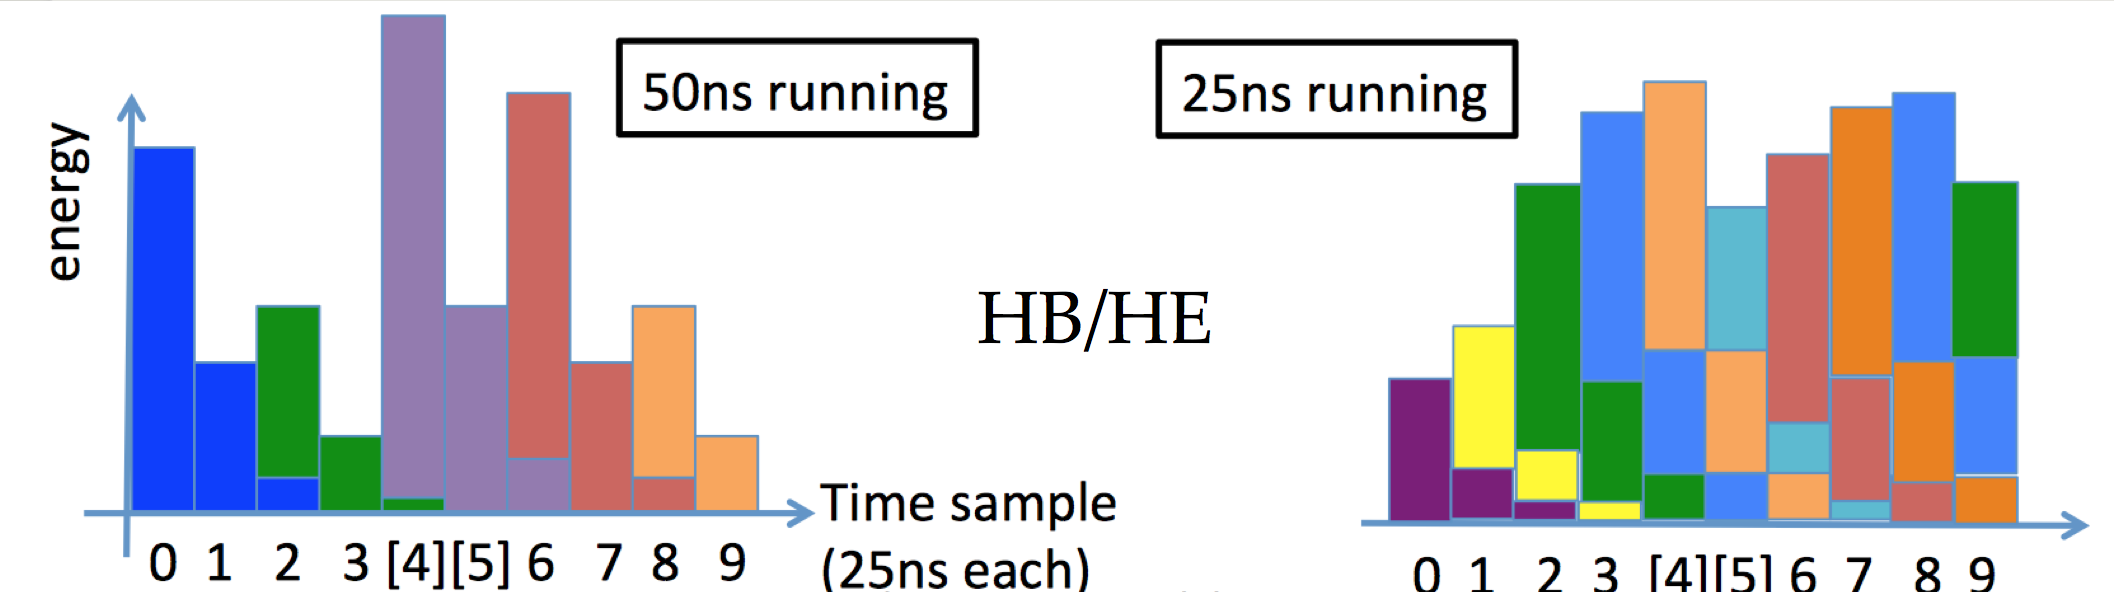
\includegraphics[width=0.8\textwidth]{fig/hcal25ns.png}
\begin{itemize}

\item Algorithm parameterizes pulse shape as function of charge in triggered TS
\label{sec-3-2-1-2}%
\begin{itemize}

\item Step 1: Measure shape in data for given $|\eta|$ regions
\label{sec-3-2-1-2-1}%

\item Step 2: Use pulse shape to subtract OOT pulses
\label{sec-3-2-1-2-2}%
\end{itemize} % ends low level

\item Status:
\label{sec-3-2-1-3}%
\begin{itemize}

\item Baseline method \alert{validated and ready} for \texttt{CMSSW\_7\_2\_0}
\label{sec-3-2-1-3-1}%

\item See \href{https://indico.cern.ch/event/318703/session/2/contribution/7/material/slides/0.pdf}{\underline{\alert{talk}}} by \href{mailto:artur.apresyan@cern.ch}{\underline{\alert{Artur Apresyan}}}
\label{sec-3-2-1-3-2}%

\item Work is not done!  New algorithms are under study!
\label{sec-3-2-1-3-3}%
\end{itemize} % ends low level
\end{itemize} % ends low level
\end{frame}
\subsection{Reconstruction: alternative method}
\label{sec-3-3}
\begin{frame}
\frametitle{Reconstruction: alternative method}
\label{sec-3-3-1}
%% Figure
\label{sec-3-3-1-1}

\centering
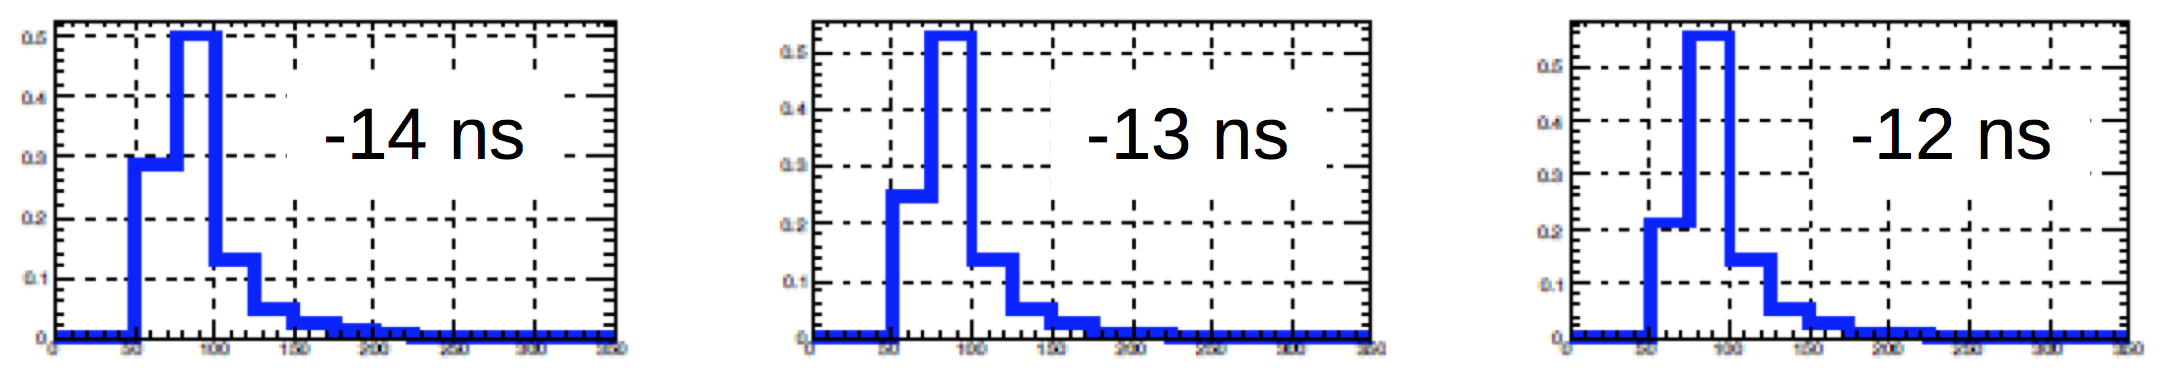
\includegraphics[width=\textwidth]{fig/hcal25_MIT.png}
\begin{itemize}

\item Also, new method being investigated by the MIT group
\label{sec-3-3-1-2}%
\begin{itemize}

\item Step 1: fit pulse shape for arrival time and total charge
\label{sec-3-3-1-2-1}%

\item Step 2: use fit to estimate the OOT PU contamination in energy when there are two pulses
\label{sec-3-3-1-2-2}%
\end{itemize} % ends low level

\item Still in development stage, but manpower is present
\label{sec-3-3-1-3}%

\item Regular status updates in HCAL reconstruction working group
\label{sec-3-3-1-4}%
\end{itemize} % ends low level
\end{frame}
\section{Noise filters}
\label{sec-4}
\subsection{Introduction to noise filters}
\label{sec-4-1}
\begin{frame}
\frametitle{Noise filters scope and priorities}
\label{sec-4-1-1}
\begin{itemize}

\item Noise filters that worked in Run 1 need to be updated for the Run 2 environment
\label{sec-4-1-1-1}%

\item These updates are under development, and the results are encouraging
\label{sec-4-1-1-2}%

\item Note that these noise filters may change a bit with the reconstruction algorithm
\label{sec-4-1-1-3}%
\end{itemize} % ends low level
\end{frame}
\begin{frame}
\frametitle{Noise filters outline}
\label{sec-4-1-2}
\begin{block}{Main areas of focus:}
\label{sec-4-1-2-1}

\begin{enumerate}
\item R45 upgrade filter
\item Negative energy filter
\item Validation on data and MC \& implementation in CMSSW
\end{enumerate}
\end{block}
\begin{itemize}

\item Convener: \href{mailto:yi.chen@cern.ch}{\underline{\alert{Yi Chen}}}
\label{sec-4-1-2-2}%
\end{itemize} % ends low level
\end{frame}
\subsection{R45 upgrade filter}
\label{sec-4-2}
\begin{frame}
\frametitle{R45 upgrade filter}
\label{sec-4-2-1}
\begin{columns} % Columns
\label{sec-4-2-1-1}
\begin{column}{0.55\textwidth}
%% Text column
\label{sec-4-2-1-1-1}
\begin{itemize}

\item \(R45 = \frac{TS4 - TS5}{TS4 + TS5}\) used in 2012 to identify RBX noise
\label{sec-4-2-1-1-1-1}%

\item New method needed for 25 ns
\label{sec-4-2-1-1-1-2}%

\item An RBX with a large fraction of energy coming from ``noisy'' RecHits is suspect
\label{sec-4-2-1-1-1-3}%

\item Initial results encouraging
\label{sec-4-2-1-1-1-4}%

\item Need more work to finalize version in CMSSW
\label{sec-4-2-1-1-1-5}%
\end{itemize} % ends low level
\end{column}
\begin{column}{0.55\textwidth}
%% Figure column
\label{sec-4-2-1-1-2}
%% Figure 1
\label{sec-4-2-1-1-2-1}

\centering
Healthy RBX
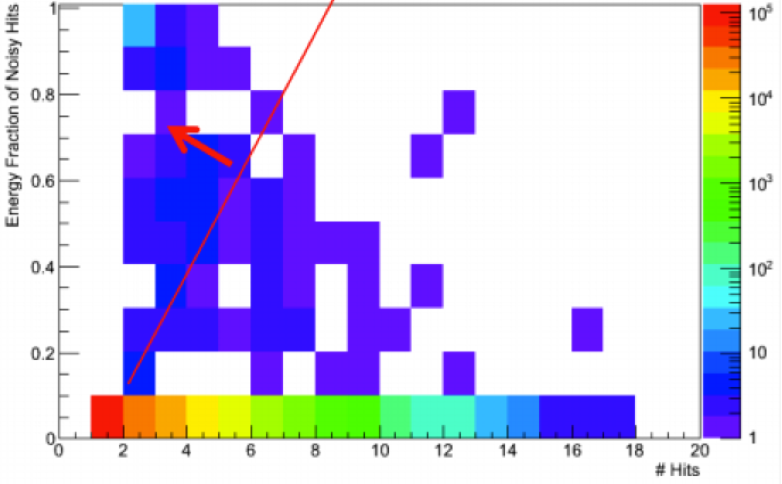
\includegraphics[width=0.7\textwidth]{fig/HealthyRBX.png}
%% Figure 2
\label{sec-4-2-1-1-2-2}

\centering
Noisy RBX
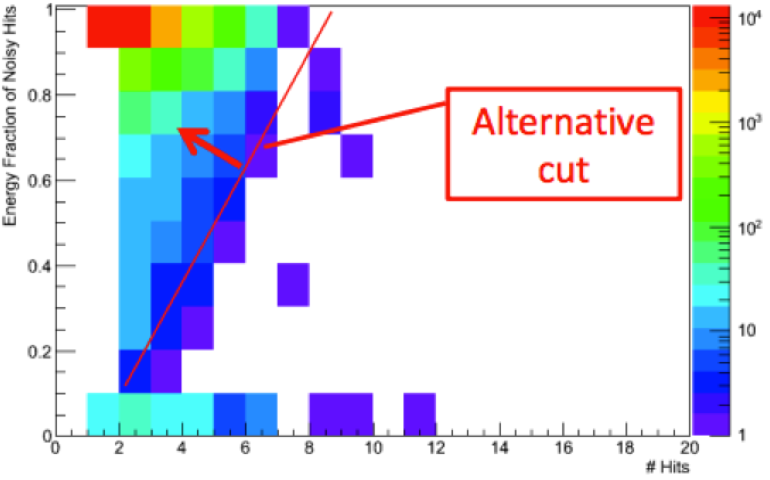
\includegraphics[width=0.7\textwidth]{fig/NoisyRBX.png}
\end{column}
\end{columns}
\end{frame}
\subsection{Negative energy filter}
\label{sec-4-3}
\begin{frame}
\frametitle{Negative energy filter}
\label{sec-4-3-1}
\begin{columns} % Columns
\label{sec-4-3-1-1}
\begin{column}{0.55\textwidth}
%% Text column
\label{sec-4-3-1-1-1}
\begin{itemize}

\item New HCAL reconstruction corrects for expected tail from previous time samples
\label{sec-4-3-1-1-1-1}%

\item For spike-like noise, reconstructed energy from TS6 can be negative
\label{sec-4-3-1-1-1-2}%

\item Initial results encouraging (see plot for data, right)
\label{sec-4-3-1-1-1-3}%

\item Need more work to finalize version in CMSSW
\label{sec-4-3-1-1-1-4}%
\end{itemize} % ends low level
\end{column}
\begin{column}{0.55\textwidth}
%% Figure column
\label{sec-4-3-1-1-2}
%% Figure 1
\label{sec-4-3-1-1-2-1}

\centering
Cartoon of effect
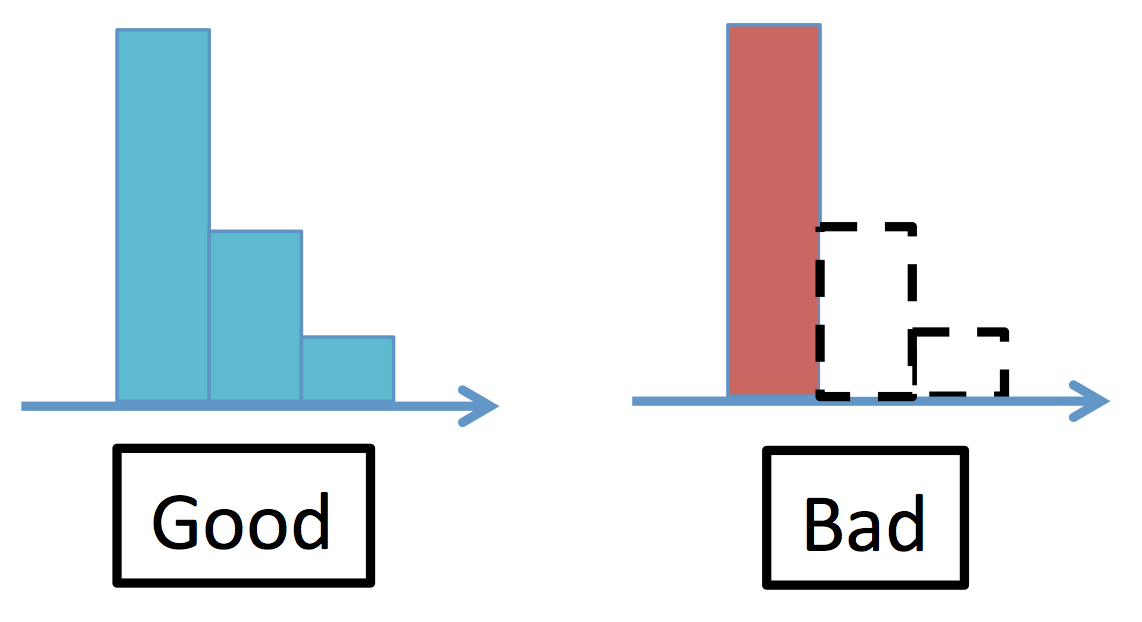
\includegraphics[width=0.7\textwidth]{fig/negative.png}
%% Figure 2
\label{sec-4-3-1-1-2-2}

\centering
OOT PU-corrected TS6 in data
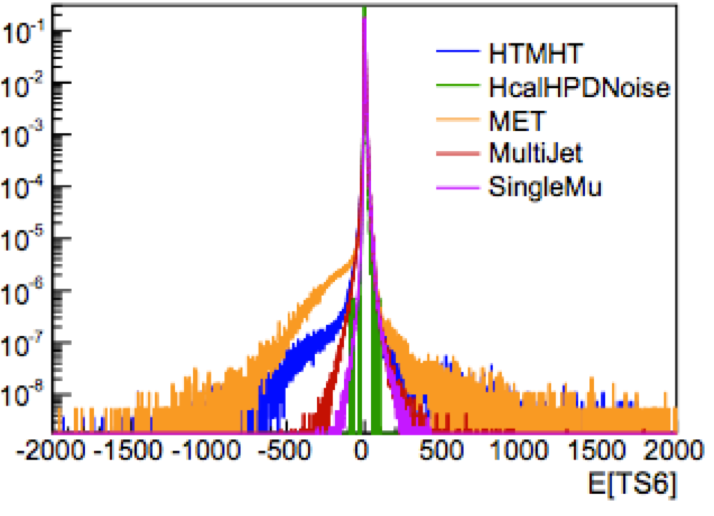
\includegraphics[width=0.7\textwidth]{fig/TS6.png}
\end{column}
\end{columns}
\end{frame}
\section{Conclusion}
\label{sec-5}
\subsection{Conclusion}
\label{sec-5-1}
\begin{frame}
\frametitle{Conclusion}
\label{sec-5-1-1}
\begin{itemize}

\item HCAL is preparing for data taking in 2015
\label{sec-5-1-1-1}%

\item Lots of new developments are underway:
\label{sec-5-1-1-2}%
\begin{itemize}

\item New/updated calibration efforts
\label{sec-5-1-1-2-1}%

\item New/updated noise filtering algorithms
\label{sec-5-1-1-2-2}%

\item New OOT PU mitigation algorithms
\label{sec-5-1-1-2-3}%
\end{itemize} % ends low level

\item Some improvements are already in place
\label{sec-5-1-1-3}%

\item Other improvements are coming soon
\label{sec-5-1-1-4}%

\item Questions are welcome
\label{sec-5-1-1-5}%
\end{itemize} % ends low level
\end{frame}

\end{document}
